\chapter{引言}

\section{研究意义}

众所周知地震灾害是关系到国计民生的重大自然灾害,虽然极具破坏的大地震发生频率很低,但是一次地震所爆发的能量却是与吨级核爆相当\citep{Stein2003},其破坏性不言而喻。如2008年5月12号的汶川地震是自唐山地震以来在我国发生的导致直接死亡人数最多,经济损失最大的重大地震,其影响震惊海内外。然而,另一方面,地震的高能量所激发的高穿透力的地震波却是地震学家研究地球结构的福音,是人类目前研究地球内部结构的最有力工具。所以,无论从人民生活安全,经济保障,还是从科学探索的角度看,地震学研究都是很有意义的。

地震学研究的主要内容包括震源以及地下结构研究,震源机制是震源最基本的参数之一,其结果可进一步应用于理论震动图计算\citep{Wald2005}、海啸模拟\citep{Satake2007}、库仑应力转移估计\citep{King2007}、区域的应力分析和震源破裂过程反演中\citep{Kilb2001}。此外,利用已知震源机制计算得到面波震动图,用于在介质结构研究中代替到时或面波频散数据,以获得更多约束信息,直接拟合实际波形反演地下结构的方法也得到了广泛应用\citep{Nolet1990,Manaman2011,Friederich2003,Zielhuis1994,Cao2001,Lee1997}。因而在地震发生后,获得可靠的震源机制是有益且必要的。

由于真实情况下,获得的观测数据质量都不是完美的,为了得到更为准确和可靠的震源机制,需要在反演过程中尽可能优化结果。理论上,在给定观测数据和目标函数情况下,对于结果的最直接调控来自于反演的权重。合理的权重能使得对现有数据中有用信息更充分的应用,并压制无效噪声对反演的干扰影响。不同的加权得到的结果往往有差异,为了反演得到更“真实”的震源机制,必须谨慎考虑,合理地为数据加权。

另一方面,因为数据中的噪声具有随机性,使得反演结果相对真值有不可准确预料的偏差。事实上,反演结果与真实值的偏差还来源于所需参考模型的误差,数值计算舍入误差,理论的近似引起的偏差等等系统性误差。在此仅关注研究数据噪声引起的误差,为了方便,本文之后所提的误差除非特别指出,否则均指数据随机噪声导致的震源机制误差。正是因为误差不可预料,为了使结果具有科学参考价值,必须对噪声可能导致的误差范围进行评估。排除数据噪声影响的“理想”结果则包含在反演结果的误差范围内,虽然无法直接求出该“理想”结果,但至少能在一定置信区间内给出可靠的结果范围,对于借鉴以及进一步深入研究均具有重要意义。此外,对于某些算法而言(如本文反演所用的格点搜索算法),无论结果是否可信反演后均会得到一个“最优解”,但当涉及病态反演问题时,该震源机制很可能与真实情况有非常大偏差,未经过误差评定,结果可能对之后研究者具有误导作用。

\section{研究发展历程}

\subsection{方法分类}

利用地震波信息反演震源机制根据反演数据源差异主要可以分为三大类方法。第一类是P波极性反演,利用了初至波第一次起跳方向信息约束震源,但对台站分布要求高,且结果不太稳定;第二类是用振幅定量信息反演,利用各震相振幅的差异或方位特性等定量信息进行反演,但续至波的振幅测量通常比较困难;第三类是波形拟合反演,直接利用整个波形数据的所有可用信息计算震源机制,约束效果相对更好。

\subsection{P波初动极性反演}

早期的震源机制反演根据P波初动极性在四象限中的分布规律\citep{Balakina1961}。这种方法首先起源于\citet{Reid1910}在1906年旧金山地震研究\citep{Milne1910}基础上提出了弹性回跳理论——认为地震是由于地壳中岩石积累了过多应变能,超过其承受能力后,发生弹性断裂,势能随之释放。之后,P波初动符号的规律被发现\citep{Nakano1923},人们提出了地震节面的概念。并开始利用地震台站记录到的地震波初动极性信息在被地震节面分隔的四象限空间的分布,对震源节面进行约束,进而得到震源机制。然而由于该方法仅使用了P波初动极性这一少量信息,并且初动极性的明显性与初动P波振幅相关。理论上P波初动极性及振幅大小所形成的辐射花样在节面分隔的四象限中分布如\reffig{fig1_01},可以发现,在节面上P波理论振幅为零。因此在节面附近,P波信号可能淹没在噪声当中,无法识别。以上原因导致该方法适用性受限,且结果不太稳定,为了得到稳定结果该方法对台站的数量和分布要求很苛刻。
\begin{figure}
\centering
  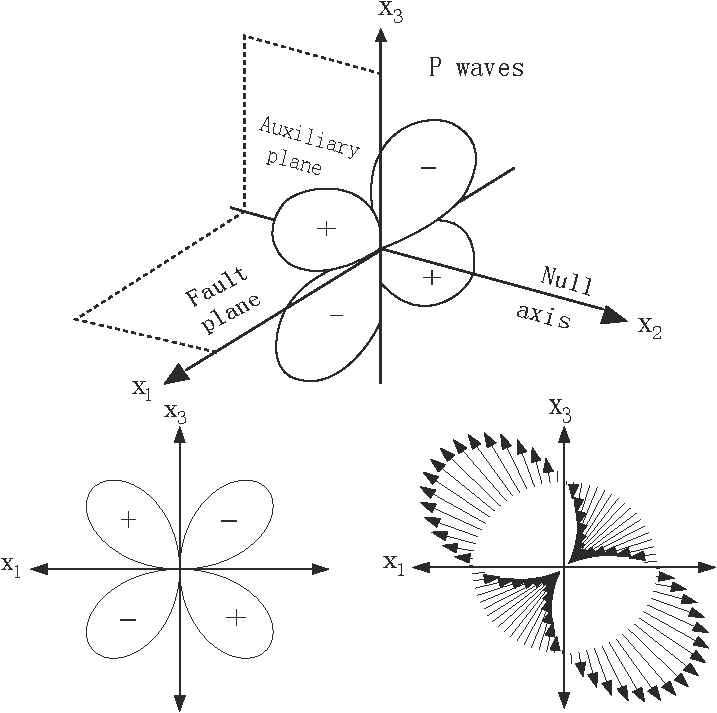
\includegraphics[scale=0.8]{fig1_01.pdf} 
  \caption{断层面($x_1$)和辅助面($x_3$)所分隔的四象限中P波辐射花样\citep{Stein2003}}
  \label{fig1_01}
\end{figure}

\subsection{振幅比反演}

第二类方法是利用各震相的振幅信息,使用波形振幅的定量数值信息,相对P波初动极性反演方法增加了反演数据的可用约束信息。这类方法包括利用P,S波的振幅比信息,通过同一台站不同分量震相信息比值规律,可一定程度避免来自介质模型不准确的系统性误差影响。其中利用P震相与SV震相的震幅比\citep{Kisslinger1982,Kisslinger1980}是一种行之有效的方案,并为了最大程度削弱介质模型对反演的影响,选择了直达上行地球表面的Z分量波。此外,在Kisslinger的研究基础上,\citet{wudaming1989}发现当有较高质量SH波时,通过P震相与SH震相的振幅比值反演可能得到相比P,SV振幅比反演更可靠的震源机制。另外,也有利用面波的振幅花样\citep{Stein2003}反演震源机制等可行方案。虽然利用振幅信息有效增强了对震源的约束,但是仍然对台站分布有较高要求,而且对近震波形S波初至振幅的测量,尤其是SV波的测量显得较为困难\citep{qiyuping2013},稍有不慎便可能得到较大偏差。

\subsection{波形拟合反演}

波形拟合反演直接利用了整个波形数据的所有信息进行反演,随着理论地震波的研究取得巨大成功\citep{Haskell1964,Herrmann1979,Wang1980}。在给定介质模型和震源机制情况下可以比较精确地计算出理论波形,使得直接使用观测波形数据与理论数据匹配反演震源机制的想法得以实现。通常波形中的体波数据由于穿透深,受浅层不均匀地壳结构影响较小,但考虑到体波衰减快,通常利用远震体波反演较大地震的震源机制,这能够减小地下介质模型横向非均匀性影响。而面波对介质结构较敏感,则较常用于具有较为精确介质参考模型的区域地震震源研究,或结合震源机制研究其较为敏感的地下结构\citep{Nolet1990}。由于波形数据相比初动极性或振幅,包含了更多有效信息,使得对台站数量及分布的要求有所降低,且结果更稳定、可靠,于是波形拟合反演的方法得到了快速发展和应用\citep{Walter1993,Ritsema1993,Zhao1994,Nabvelek1995}。

用地震波形拟合反演震源机制时,由于待求参数少、解空间有限且观测方程直接求解比较复杂,所以该问题非常适合用非线性反演中的全局搜索算法。在实践中,得到广泛应用的CAP(Cut and Paste的简称)\citep{Zhao1994,Zhu1996,Tan2006}和CPS(Computer Programs in Seismology的简称)\citep{Herrmann1989}等波形拟合反演程序充分说明了全局搜索在震源机制反演问题中的有效性。

\section{研究现状及问题}

Herrmann开发的CPS软件包中用于震源机制反演的子程序和CAP均利用格点搜索方法反演震源机制,由于二者的实用性和开源性,被广泛应用于震源机制研究中。然而CAP和CPS加权方法的侧重点不同,前者考虑几何扩散导致波形振幅的衰减,给较低振幅的波形加大权重,以平衡不同振幅波形在反演中的影响力;后者则关注传播过程中信噪比的降低,赋予高信噪比数据较大权重。进一步考虑到波形振幅及信噪比与震中距间的关系,\citet{Zhu1996}在CAP中将权重设置为关于震中距递增的幂函数,而CPS方法中使用震中距的反比例函数作为权重值。幂函数和反比例函数的单调性恰巧相反,导致从数值上看,两种方法对同一套数据波形所定权重大小相互矛盾——CPS定权震中距较近台站权重较高,而CAP定权中则震中距较远台站相对权重较大。此外,通过实例计算及理论分析发现,实际观测波形的振幅及信噪比与震中距的关系较为复杂,难以用简单的初等函数进行描述,因此利用幂函数或反比例函数估算的振幅和信噪比均较粗糙。且由于函数中包含的某些辅助参数赋值因人而异,故无法准确体现数据的真实性和客观性。

另一方面,随着CAP、CPS等用波形非线性反演震源机制的算法得到广泛应用\citep{Luo2015,DAmico2014},其非线性反演中误差缺失的问题逐渐受到关注。考虑到误差评价的重要性,国内外学者均对震源机制反演的误差估计问题进行了研究,\citet{Duputel2012}从误差的来源入手,对震源机制进行误差评价,但其方法只适用于线性反演的震源机制误差估计。考虑到目前应用广泛的全局搜索反演,本文旨在探究能应用于非性线反演算法的误差评估方法。对于非线性反演,最常见的方法是对目标函数的极值人为给定一个阈值,满足该条件的所有解构成误差范围内解集,该方法简洁直观,能快速发现不同模型参数的误差相对大小关系,但是阈值的给定有主观性,导致定量结果难以让人信服。\citet{zhenjianchang2015}借鉴Bootstrap(Efron1979)的思想,对数据集随机多次选取子集进行独立反演并对解集样本用一定方法分析,以评估其整体误差及解。但是为使样本能反映整体,统计分析不仅要求样本抽取的随机性,还对原始样本大小有一定要求,当可用的地震记录数量不是很大时,可随机选择的子样本以及子样本总量难以满足统计要求,基于重抽样的该方法便不适用了。

\section{本文设定目标及方案}

针对以上分析,为了解决CPS和CAP反演定权方法出现的矛盾以及误差缺失问题,本文分别尝试进行权重优化以及误差评定。对于定权,结合CPS与CAP,综合考虑振幅衰减和信噪比差异影响,将二者统一计算权重,从而解决上述的权重数值矛盾问题。其次,计算时摈弃了用震中距简单函数估算振幅或信噪比方案,而是基于每道波形数据自身的信息,准确评估振幅和噪声。由于没有人工干预,在提高精确度的同时有效保证了客观性。

针对反演震源机制时欠缺误差估计的问题,本文借鉴了\citet{Hardebeck2002}对P波初动极性反演方法改进的思路——首先估计观测数据的随机误差大小,据此模拟随机误差,并将其加入原始数据生成多组模拟数据集,最终反演得到一系列误差范围内的解集。该方法不仅估计了误差,且使得反演结果更稳定\citep{Hardebeck2002}。将该思想应用到波形反演震源机制的问题中,通过评估噪声随机模拟多套波形数据集,并用每套数据分别独立进行反演,得到包含多个反演结果的解集,最后对解集统计分析得到解的误差。本文方法与\citet{zhenjianchang2015}的重采样类方法不同的是每次反演的数据并非原始数据集的子集,而是与数据集等价的模拟数据集,保留了原数据集的样本大小,更重要的是每套数据均具有一致的数据分布结构。对观测数据的数量要求相对降低,理论上能比重采样类方法更好应用于台站记录较稀少的地震事件。

为了验证本文提出权重优化方案和误差评价方法的有效性,基于CPS反演程序进行了一系列理论试验,分别检验权重优化效果和误差估计与理论预测是否吻合。对同一个设定条件下的模拟地震进行了三次试验,分别测试权重优化的效果,误差评定方法对噪声的反应情况,误差评价时重复反演次数的设定值。第一次试验分别设定了单独信噪比加权,单独振幅调节加权,信噪比和振幅调节联合定权三组对照组。三组反演组结果相差不大,但联合反演组的综合偏差更小,体现了联合定权的优越性。第二次试验测试结果误差对数据噪声的反应是否合理,以证明误差估计方法的有效性,对理论事件加噪时分别加了低、中、高及超高强度噪声,反演结果确实体现了误差由低到高的趋势,而且增长率符合理论预测。理论真值均在各次反演的误差范围内,表明了本文误差估计结果的真实性。第三次试验研究误差评价时反演的重复次数对最终结果的影响,用以为该方法在应用时选择合适的反演次数。试验分别尝试了重复10次,50次,100次和200次,结果发现该方法在次数达到50次-200次之间对反演次数不是特别敏感,结果基本一致且可信。为同时保证样本量充足并节省计算时间,选定100次为默认反演次数。

为了体现本文方法的实际应用性,以2013年4月20日的芦山地震为例,分别采取单独振幅调节加权、单独信噪比加权以及振幅调节和信噪比调节联合加权的策略进行三次反演,并利用本文的误差估计方法对三次反演的结果进行评价。通过对结果的合理可靠性及稳定性两方面进行综合讨论比较,以真实案例证实本文联合加权策略反演结果最优,最终振幅调节和信噪比调节联合加权对应的震源机制解为(走向$211\degree\pm5\degree$,倾角$41\degree\pm1\degree$,滑动角$94\degree\pm2\degree$),震源深度17km,与其它研究者的研究成果有很好的一致性,且与震源区的应力及地质构造情况均相互吻合。
